\section{Differential Evolution}
\label{sec:de}

Differential evolution (DE)~\cite{storn1997differential} is a population based search metaheuristic designed to iteratively improve candidate solutions to a problem. DE is well suited for problems containing a nonlinear and non-differentiable continuous search space. DE works by creating a new candidate solution using existing candidate solutions in the population using a \textit{mutation} operator. Once a new candidate solution is created the fitness scores of each solution are compared and the candidate with the better fitness score is put into the new population. Candidate solutions in DE are refered to as \textit{agents}. Figure~\ref{fig:deFlowchart} depicts how evolution occurs in DE and Subsections~\ref{subsec:de-mutation} and~\ref{subsec:de-selection} describe the operators used.

% \begin{figure}[H]
%   \centering
%   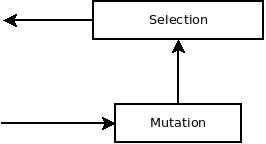
\includegraphics[bb=0 0 266 144,scale=0.5]{figures/DE.jpeg}
%   \caption{DE Evolution}
%   \label{fig:deFlowchart}
% \end{figure}

% \subsection{Agents}

The candidate solutions found in the population of a DE are referred to as agents. Each agent contains a vector of real numbers which represents its position within the search space.

\subsection{Mutation}
\label{subsec:de-mutation}

The mutation operator is used to create new individuals from the existing individuals. Individuals are combined using the mathematical formula, shown in Algorithm~\ref{alg:de-mutation}, to create new individuals. Algorithm~\ref{alg:de-mutation} describes the pseudocode for the mutation operator. The mutation operator is performed once for each agent in the population. To locate a new agent's position first three different agents must be randomly selected from the population. The agent's position is combined with the three other agents' positions to create a new position. Each position index within the agent is updated either based on the three other agents selected or the value from the previous agent is copied. The new agent's position is evaluated based on the fitness function. If the agent's new position has resulted in an improved fitness score the new position replaces the old one. If not, the new position is discarded. The variable $F \in [0,2]$ is known as the differential weight, and variable $CR \in [0,1]$ is known as the crossover probability. Both of these variables are user defined.

\begin{algorithm}
	\caption{Mutation}
	\label{alg:de-mutation}
	\begin{algorithmic}

		\FOR{each agent $X$ in the population}
			\STATE{pick three agents $a$, $b$, $c$ randomly from the population}
			\STATE{pick random index $R \in \{1, \ldots, n\}$}
			\STATE{copy agent $X_i$ to $y$}
			\FOR{each position index $y_j$ in $[y_1, \ldots, y_n]$}
				\STATE{$r_j = U(0,1)$}
				\IF{$r_j < CR$ or $R == j$}
					\STATE{$y_j = a_j + F(b_j - c_j)$}
				\ELSE
					\STATE{$y_j = {X_i}_j$}
				\ENDIF
			\ENDFOR
			\IF{$f(y) < f(X_i)$}
				\STATE{$X_i = y$}
			\ENDIF
		\ENDFOR

	\end{algorithmic}
\end{algorithm}

% \subsection{Selection}
% \label{subsec:de-selection}

% The selection operator determines whether the newly created agent from the mutation operator should be placed in the new population of candidate individuals. Once the new agent is created it is evaluated based on the evaluation function described in Subsection~\ref{subsec:fitness-function}. If the new agent has an improved fitness score over the original agent, the new agent is placed in the new population. Otherwise, the original agent is placed in the new population.
